\subsection{Search}
This subsection will allow users to search for playlists on their music accounts through Synthify.

\begin{figure}[h!]
	\centering
 	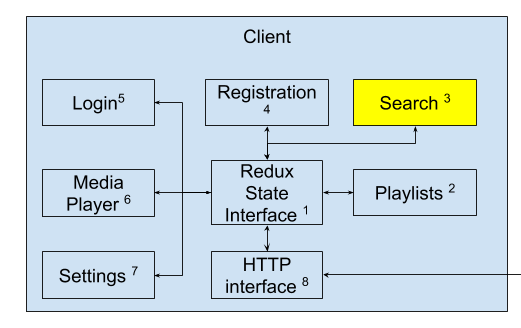
\includegraphics[width=0.60\textwidth]{images/client/client_search.png}
 	\caption{Search subsystem}
\end{figure}

\subsubsection{Assumptions}
We are assuming that the user has at least one account connected to Synthify.

\subsubsection{Responsibilities}
Responsibilities include displaying results (playlists based on user's search term) for the users and a search bar allowing a user to type in their search term.

\subsubsection{Subsystem Interfaces}
\begin {table}[H]
\caption {Search interfaces} 
\begin{center}
    \begin{tabular}{ | p{1cm} | p{6cm} | p{3cm} | p{3cm} |}
    \hline
    ID & Description & Inputs & Outputs \\ \hline
    \#1 & Redux State Interface & \pbox{3cm}{Search Term} & \pbox{3cm}{List of playlists}  \\ \hline
    \end{tabular}
\end{center}
\end{table}

\newpage
